\clearpage
\setcounter{section}{0}

\section*{Lesson 2: Integers ($\mathbb{Z}$)}


\subsection*{វត្ថុបំណងនៃការសិក្សា}
នៅចុងបញ្ចប់នៃមេរៀននេះ សិស្សនឹងអាច៖
\begin{itemize}[label=---]
    \item កំណត់និយមន័យចំនួនគត់។
    \item តាងចំនួនគត់នៅលើបន្ទាត់ចំនួន។
    \item ប្រៀបធៀប និងរៀបលំដាប់ចំនួនគត់។
    \item អនុវត្តប្រមាណវិធីបូក ដក គុណ និងចែកជាមួយចំនួនគត់។
\end{itemize}

\section{គោលគំនិតសំខាន់ៗ}
\subsection{តើអ្វីជាចំនួនគត់?}
ចំនួនគត់រួមមានចំនួនគត់ធម្មជាតិ, សូន្យ, និងចំនួនគត់អវិជ្ជមាន៖ $\{\dots, -3, -2, -1, 0, 1, 2, 3, \dots\}$ ។

\subsection{បន្ទាត់ចំនួន}
\begin{figure}[h!]
    \centering
    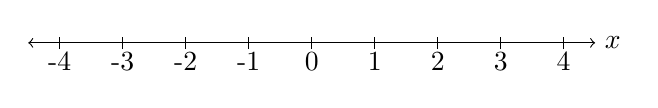
\begin{tikzpicture}[scale=0.8]
        \draw[<->] (-4.5,0) -- (4.5,0) node[right] {$x$};
        \foreach \x in {-4,-3,-2,-1,0,1,2,3,4} {
            \draw (\x, -0.1) -- (\x, 0.1);
            \node at (\x, -0.3) {\x};
        }
    \end{tikzpicture}
    \caption{បន្ទាត់ចំនួនបង្ហាញពីទីតាំងនៃចំនួនគត់។}
    \label{fig:integer-number-line}
\end{figure}

\subsection{ប្រមាណវិធីលើចំនួនគត់}
\subsubsection{ការបូកចំនួនគត់}
\begin{itemize}
    \item \textbf{សញ្ញាដូចគ្នា៖} បូកតម្លៃដាច់ខាតរបស់វា ហើយរក្សាសញ្ញារួម។\\
    ឧទាហរណ៍៖ $(-3) + (-5) = -8$
    \item \textbf{សញ្ញាផ្ទុយគ្នា៖} ដកតម្លៃដាច់ខាតតូចជាងចេញពីតម្លៃដាច់ខាតធំជាង ហើយយកសញ្ញាតាមចំនួនដែលមានតម្លៃដាច់ខាតធំជាង។\\
    ឧទាហរណ៍៖ $(-7) + 4 = -3$
\end{itemize}

\subsubsection{ការដកចំនួនគត់}
ដើម្បីដកចំនួនគត់មួយ, ត្រូវបូកនឹងចំនួនផ្ទុយរបស់វា ($a - b = a + (-b)$)។\\
ឧទាហរណ៍៖ $5 - (-3) = 5 + 3 = 8$

\subsubsection{ការគុណចំនួនគត់}
\begin{itemize}
    \item \textbf{សញ្ញាដូចគ្នា៖} ផលគុណជាចំនួនវិជ្ជមាន។\\
    ឧទាហរណ៍៖ $(-4) \times (-2) = 8$
    \item \textbf{សញ្ញាផ្ទុយគ្នា៖} ផលគុណជាចំនួនអវិជ្ជមាន។\\
    ឧទាហរណ៍៖ $(-6) \times 3 = -18$
\end{itemize}

\subsubsection{ការចែកចំនួនគត់}
\begin{itemize}
    \item \textbf{សញ្ញាដូចគ្នា៖} ផលចែកជាចំនួនវិជ្ជមាន។\\
    ឧទាហរណ៍៖ $(-10) \div (-2) = 5$
    \item \textbf{សញ្ញាផ្ទុយគ្នា៖} ផលចែកជាចំនួនអវិជ្ជមាន។\\
    ឧទាហរណ៍៖ $15 \div (-3) = -5$
\end{itemize}

\section{ឧទាហរណ៍អនុវត្ត}

\begin{example}{ការប្រៀបធៀបចំនួនគត់}
    តើមួយណាធំជាង, $-5$ ឬ $-2$?
    \begin{solution}
        នៅលើបន្ទាត់ចំនួន, $-2$ នៅខាងស្តាំ $-5$, ដូច្នេះ $-2 > -5$។
    \end{solution}
\end{example}

\begin{example}{ការបូក និងដកចំនួនគត់}
    គណនា៖ $(-8) + 3 - (-4)$។
    \begin{solution}
        $(-8) + 3 - (-4) = (-5) + 4 = -1$។
    \end{solution}
\end{example}

\section{លំហាត់អនុវត្ត}
\begin{enumerate}[label=\arabic*.]
    \item ប្រៀបធៀប៖ $-10$ និង $1$។
    \item គណនា៖ $(-3) + 5$។
    \item គណនា៖ $7 - (-2)$។
    \item គណនា៖ $(-5) \times (-3)$។
    \item គណនា៖ $20 \div (-4)$។
\end{enumerate}
